\chapter{Graph theory}

  \section{Definitions}
        
    \subsection{Graph}

      A graph $G$ is a pair of sets $(V, E)$ such that $E \subseteq [V]^2$. $V$ or $V(G)$ is a set of arbitrary objects called \emph{vertices} (singular is \emph{vertex}) or \emph{nodes}, while $E$ or $E(G)$ is a set of vertex pairs, called \emph{edges} or \emph{arcs} on occasion; elements of $E$ are two-element subsets of $V$\cite{Diestel2012}.
      
      There are two graph types in respect to edge type: \emph{undirected} and \emph{directed}, pictured on figure \ref{fig:graphs_orientation_undirected} and \ref{fig:graphs_orientation_directed} respectively. In the former, edges are ordered pairs of vertices, i.e. $e = (u, v) = (v, u)$. In the latter they are unordered or just sets of two vertices, that is $e = (u, v) \neq (v, u) = d$.
      \begin{figure}[H]
        \centering        
          \begin{subfigure}[b]{0.25\textwidth}
            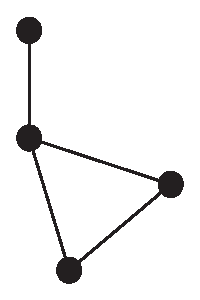
\includegraphics[width=\textwidth]{chapters/02_problem_definition/graph_undirected}
            \caption{An undirected graph.}
            \label{fig:graphs_orientation_undirected}
          \end{subfigure}
          \qquad\qquad\qquad
          \begin{subfigure}[b]{0.25\textwidth}
            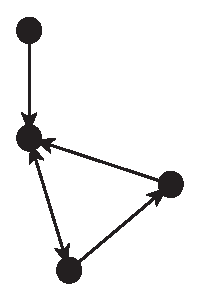
\includegraphics[width=\textwidth]{chapters/02_problem_definition/graph_directed}
            \caption{A directed graph.}
            \label{fig:graphs_orientation_directed}
          \end{subfigure}
        \caption{Types of graphs in respect to orientation.}
        \label{fig:graphs_orientation}
      \end{figure}
      
      Then we have \emph{simple graphs}, where there are no edges from a vertex to itself (called loops) and there are no more than one edge between any two distinct vertices (i.e. edges form sets). On the other side we have \emph{multigraphs} (or \emph{pseudographs}), that may both have loops (not everyone agrees with that) and multiple edges (also called parallel edges) between different vertices (thus they form a multiset).
      \begin{figure}[H]
        \centering        
          \begin{subfigure}[b]{0.25\textwidth}
            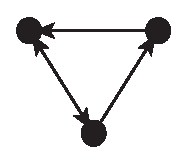
\includegraphics[width=\textwidth]{chapters/02_problem_definition/graph_simple}
            \caption{A simple graph.}
            \label{fig:graphs_simple}
          \end{subfigure}
          \qquad\qquad\qquad
          \begin{subfigure}[b]{0.25\textwidth}
            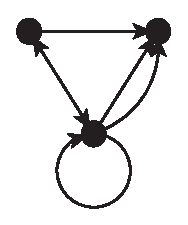
\includegraphics[width=\textwidth]{chapters/02_problem_definition/graph_multi}
            \caption{A multigraph.}
            \label{fig:graphs_multi}
          \end{subfigure}
        \caption{Types of graphs in respect to edge distinctness.}
        \label{fig:graphs_types}
      \end{figure}

      If $(u, v)$ is an edge in an undirected graph then we call $u$ a \emph{neighbour} of $v$ and vice versa. Then we call the number of such neighbours a \emph{degree} of a vertex. In directed graphs however, if $u \rightarrow v$ is a directed edge, then we call $u$ the \emph{predecessor} of $v$, which in turn we call a \emph{successor} of $u$. The \emph{in-degree} of a vertex is the number of predecessors and the \emph{out-degree} of a node is the number of its successors. It is important to note that given $u$ and $v$ and if $u \rightarrow v$ and $v \rightarrow u$ then $u \leftrightarrow v$.

      A graph $H = (U, D)$ is a \emph{subgraph} of $G = (V, E)$ if $U \subseteq V$ and $D \subseteq E$.

    \subsection{Paths}

      \subsubsection{Path}

        A \emph{path} is a sequence of edges where each successive edge share a vertex and all other edges have no vertices in common.

      \subsubsection{Cycle}

        A \emph{cycle} is a path which starts and ends at the same vertex and has at least one edge.
        
      \begin{figure}[H]
        \centering
        \begin{minipage}[b]{0.43\textwidth}
          \centering
          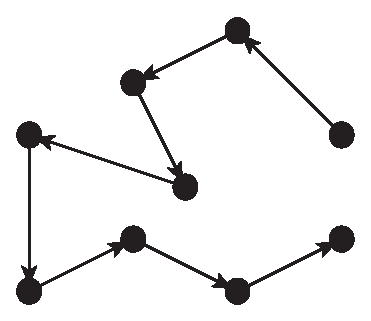
\includegraphics[width=\textwidth]{chapters/02_problem_definition/path}
          \captionof{figure}{A path.}
          \label{fig:path}
        \end{minipage}
        \qquad\qquad
        \begin{minipage}[b]{0.3\textwidth}
          \centering
          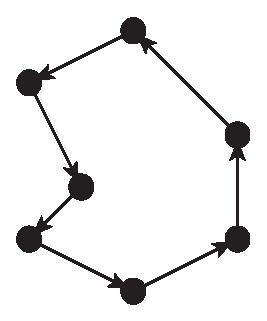
\includegraphics[width=\textwidth]{chapters/02_problem_definition/cycle}
          \captionof{figure}{A cycle.}
          \label{fig:cycle}
        \end{minipage}
      \end{figure}

      \subsubsection{Tree}

        A \emph{tree} is a special graph that is a connected acyclic graph. A tree is also a minimal connected graph, meaning that removing any of the edges will make the graph disconnected.

      \subsubsection{Spanning tree}

        A \emph{spanning tree} of graph $G$ is a subgraph that is a tree and contains all vertices of $G$. Obviously, no spanning trees exist for disconnected graphs.
        
      \begin{figure}[H]
        \centering
        \begin{minipage}[b]{0.35\textwidth}
          \centering
          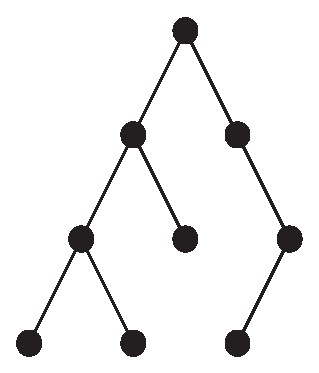
\includegraphics[width=\textwidth]{chapters/02_problem_definition/tree}
          \captionof{figure}{A tree.}
          \label{fig:tree}
        \end{minipage}
        \qquad
        \begin{minipage}[b]{0.55\textwidth}
          \centering
          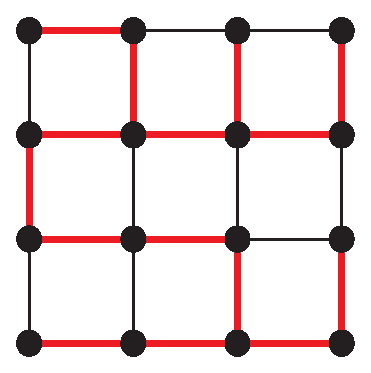
\includegraphics[width=0.7\textwidth]{chapters/02_problem_definition/tree_spanning}
          \captionof{figure}{Spanning tree (bold edges) of grid graph.}
          \label{fig:tree_spanning}
        \end{minipage}
      \end{figure}
    
    \subsection{Weighted graph}
    
      A \emph{weighted graph} is a graph that associates a label---called \emph{weight}---with every edge in the graph. Weights of edges are usually represented with real numbers. The \emph{weight of a path} in such graph is the sum of the edge weights of the edges forming a path. A non-edge has sometimes a special weight assigned with a value of infinity. Weight can also represent \emph{costs}, then words are used instead of numeric weight. A graph is always assumed to be unweighted unless otherwise has been stated.
    
    \subsection{Graph isomorphism}
        
      An \emph{isomorphism} of graphs $G$ and $H$ is a bijection between the vertices of $G$ and $H$
      \begin{equation}
        f: V(G) \rightarrow V(H)\mbox{,}
      \end{equation}
      such that an edge exists between any two vertices $u$ and $v$ of $G$ if and only if an edge exists between $f(u)$ and $f(v)$ in graph $H$. A correspondence of this kind is commonly called \textquote{edge-preserving bijection,} where isomorphisms are \textquote{structure-preserving bijections} in general notion.
        
      The above definition assumes that graphs are undirected and unweighted. However, a different definitions of isomorphism may be applied to other types of graphs, by adding the requirements to preserve the corresponding additional elements of structure like link directions, weights, \emph{etc.}, with the following exception in respect to graph labelling. If labels in graph are uniquely taken from the integer range $1,\ldots,n$, where $n$ is the number of the vertices of the graph, two labeled graphs will be isomorphic if the corresponding underlying unlabelled graphs are isomorphic.
      \begin{table}[H]
        \centering
        \begin{minipage}[b]{0.3\textwidth}
          \centering
          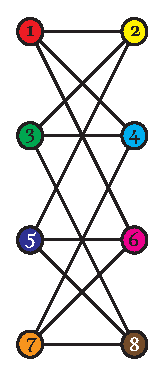
\includegraphics[width=0.55\textwidth]{chapters/02_problem_definition/isomorphism_1}
          \captionof{figure}{Graph $G$.}
        \end{minipage}
        \quad
        \begin{minipage}[b]{0.3\textwidth}
          \centering
          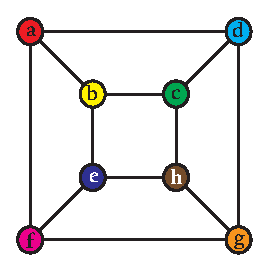
\includegraphics[width=\textwidth]{chapters/02_problem_definition/isomorphism_2}
          \captionof{figure}{Graph $H$.}
        \end{minipage}
        \qquad
        \begin{minipage}[b]{0.3\textwidth}
          \begin{tabularx}{\textwidth}{|C{1}|} \hline
          \rowcolor[gray]{0.75} $f: V(G) \rightarrow V(H)$\\\hline
            $f(1) = a$ \\\hline
            $f(2) = b$ \\\hline
            $f(3) = c$ \\\hline
            $f(4) = d$ \\\hline
            $f(5) = e$ \\\hline
            $f(6) = f$ \\\hline
            $f(7) = g$ \\\hline
            $f(8) = h$ \\\hline
          \end{tabularx}
          \caption{An isomorphism between $G$ and $H$.}
        \end{minipage}
      \end{table}
      
      The concept of \emph{graph isomorphism} makes it possible to characterise graph properties essential to the structure of the graphs themselves from properties associated with graph representations like graph drawings or data structures for graphs and labelings, \emph{etc}. For example, if a graph has exactly one cycle, then all graphs in its isomorphism class\footnote{A collection of graphs isomorphic to each other.} also have exactly one cycle. On the other hand, in the common case when the vertices of a graph are (represented by) the integers $1, 2, \ldots, N$, then the expression
      \begin{equation}
        \sum_{v \in V(G)} v\cdot\mbox{deg} v\mbox{,}
      \end{equation}
      may be different for two isomorphic graphs. But that was mentioned as an exception to the general definition.

    \subsection{Graph properties}

      In order to focus on the abstract structure of graphs, we define \emph{graph properties} as maintained under all possible \emph{isomorphisms} of a graph. However, there is a distinction referred to this term; specifically, a \emph{property} is usually referred to descriptive characterisations of graphs (i.e. it is a class of graphs), while \emph{invariant} is used for properties expressed quantitatively (i.e. it is a function from graphs to some other set, like $\mathbb{N}$). To avoid naming collisions, from now on I will mention only properties and invariants in the former sense. 

      \subsubsection{Graph invariants}

        \paragraph{Order}

          The \emph{order} of a graph is the number of vertices in a graph and is denoted by $|V(G)|$ or $|G|$.
            
        \paragraph{Size}

          The \emph{size} of a graph is the number of its edges\cite{Harris2000} in a graph and is denoted by $|E(G)|$ or $||G||$. In an undirected graph, there are $0 \leq E \leq \binom{V}{2}$ and in directed graph: $0 \leq E \leq V(V-1)$. 

        \paragraph{Eccentricity}    

          The \emph{eccentricity} $\epsilon(v)$ of vertex $v$ is the greatest geodesic distance between $v$ and any other vertex.    
                    
        \paragraph{Radius}

          The \emph{radius} $r$ of a graph is the minimum eccentricity of any vertex in the graph.

        \paragraph{Diameter}
        
          The longest of the shortest path lengths is the \emph{diameter} $d$ of a graph. It is the maximum eccentricity of any vertex in the graph. In order to find it, one first need to find the shortest path between each pair of vertices; then the greatest length of any of these paths would be the diameter of the graph.

      \subsubsection{Graph properties}

        \paragraph{Connected}

          Let $G = (V, E)$ be a graph. A non-empty graph $G$ is \emph{connected} if any two of its vertices are linked by a path in $G$, i.e. 
          \begin{equation}
            \forall_{i,j \in \mathbb{N} \cap i,j < |G|} \forall_{v_i \in V} \exists_{v_j \in V} (v_i, v_j) \in E\mbox{.}
          \end{equation}
          In other words, we call a graph \emph{connected} if there is a path from any vertex to any other vertex.

          A maximal connected subgraph of $G$ is a \emph{component} of $G$. The empty graph has no components since connected graphs are non-empty. 

          A graph that is \emph{disconnected} consists of several \emph{connected components}. Two vertices are considered to be in the same conencted component if there is a path between them.

          $G$ is called $k$\emph{-connected} (for $k \in \mathbb{N}$) if $k < |G|$ and $G - X$ is connected for every $X \subseteq V$ with $k > |X|$. Every non-empty graph is 0-connected and 1-connected graphs are precisely non-trivial connected graphs. The greatest integer $k$ such that $G$ is $k$-connected is the \emph{connectivity} $\kappa(G)$ of $G$. Hence graph is disconnected if and only if $\kappa(G) = 0$. The simplest 2-connected graphs are the cycles; all the others can be inductively constructed by adding paths to cycles.

        \paragraph{Cyclic}
        
          Graph is cyclic when it consists of a single cycle.
          
        \paragraph{Acyclic}
        
          A graph is called acyclic if there are no subgraphs that are cycles.

        \paragraph{Bipartite}
        
          We call a graph a \emph{bipartite} or a \emph{bigraph} if a graph has vertices can be divided into two disjoint sets $U$ and $V$ such that the edges only exists between independent vertices in $U$ and $V$ and never between vertices of the same set\cite{Diestel2012}. Equivalent defeinition is that a bipartite graph is a graph that does not contain any cycles with odd lengths\cite{AsratianDenleyHaggkvist}. An example of bipartite graph is presented on figure \ref{fig:cs_network} in section \ref{sec:cs}.

          The two sets $U$ and $V$ may be thought of as a colouring of the graph with two colours: if one colours all nodes in U blue, and all nodes in V green, each edge has endpoints of differing colours, as is required in the graph colouring problem\cite{AsratianDenleyHaggkvist,Scheinerman2012}. In contrast, such a colouring is impossible in the case of a non-bipartite graph, such as a triangle: after one node is coloured blue and another green, the third vertex of the triangle is connected to vertices of both colours, preventing it from being assigned either colour.
          
          A bigraph with partition sets $U$ and $V$ with $E$ denoting edges of the graph is often written as $G=(U,V,E)$. If such graph is disconnected, it may have more than one bipartition;\cite{ChartrandZhang2008}. In this case, the $(U,V,E)$ notation is helpful in specifying one particular bipartition that may be of importance in an application.
          
          Bipartite graphs very often arise naturally when dealing with real-world examples. For instance, a graph of movie actors and movies, with an edge between an actor and a movie if the actor has starred in that movie. It is a classic example of an affiliation network, which is a type of bigraph used in analysis of social networks\cite{WassermanFaust1994}.

  \section{Graphs representation}

    Graphs are usually visualised as \emph{embeddings}. An embedding of a graph $G(V, E)$ is representation of $G$ on $\Sigma$ plane in which all $v \in V$ are associated to points on $\Sigma$ and each of $e \in E$ are arcs or straight line segments between points corresponding to vertices at both ends of $e$. If no two arcs ever intersect, the embedding of a graph is called \emph{planar}, otherwise it is called a \emph{non-planar}. Because the same graph can have many embeddings that are different, it is important not to confuse the particular embedding with a graph itself. In particular, planar graphs can have non-planar embeddings too.

    There are many other ways of graph visualisation, but apart from the above and below, they are not useful for analysis of the data that is a subject of this thesis.

    Graphs can be explicitly represented by either \emph{adjacency matrices} or \emph{adjacency lists}.
        
    The adjacency matrix of a graph $G$ is a $|V| \times |V|$ matrix of indicator variables. Each entry in this matrix indicates whether a particular edge between indexes is or is not in graph $G$:
    \begin{equation}
      A[i, j] = [(i, j) \in E] \mbox{.}
    \end{equation}
    For undirected graph, similar to the edges, the adjacency matrix is always symmetric: $A[i, j] = A[j, i]$. In simple graphs, diagonal entries in $A$ are all zeros since loops are not allowed. The most valuable property of adjacency matrix is that we can decide in $\Theta(1)$ time whether two arbitrary vertices are connected by an edge just by looking at the appropriate elements of the matrix. We also can scan for a list of all vertex neighbours by looking at the corresponding row (or column), which will require $\Theta(V)$ time. The main disadvantage is that this matrix will always take $\Theta(V^2)$ space regardless of how many edges the graph really have. This makes adjacency matrices efficient for \emph{dense} graphs.
    \begin{table}[H]
        \centering
        \begin{minipage}[b]{0.3\textwidth}
          \centering
          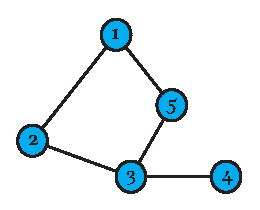
\includegraphics[width=0.8\textwidth]{chapters/02_problem_definition/adjacency}
          \captionof{figure}{Graph $G$.}
        \end{minipage}
        \quad
        \begin{minipage}[b]{0.33\textwidth}
          $$\begin{pmatrix}
            0 & 1 & 0 & 0 & 1 \\
            1 & 0 & 1 & 0 & 0 \\
            0 & 1 & 0 & 1 & 1 \\
            0 & 0 & 1 & 0 & 0 \\
            1 & 0 & 1 & 0 & 0
          \end{pmatrix}$$
          \captionof{figure}{Adjacency matrix.}
        \end{minipage}
        \qquad
        \begin{minipage}[b]{0.27\textwidth}
          \begin{tabularx}{\textwidth}{L{1}}
            $1 \to 2,\,5$ \\
            $2 \to 1,\,3$ \\
            $3 \to 2,\,4,\,5$ \\
            $4 \to 3$ \\
            $5 \to 1,\,3$
          \end{tabularx}
          \caption{Adjacency list.}
        \end{minipage}
      \end{table}

    On the other hand, adjacency lists are good when dealing with \emph{sparse} graphs (graphs with relatively small number of edges). Adjacency list is an array of linked lists (one per vertex). For undirected graphs each edge $(u, v)$ is stored twice: once in $u\mbox{'s}$ neighbourhood and once in $v\mbox{'s}$ neighbour list. For directed graph each edge is stored only once. Either way, adjacency list will take $O(V+E)$ space; listing all the neighbours of $v$ vertex takes $O(1+deg(v))$ time (by scanning the neighbour list). We can determine whether $(u, v)$ is an edge by scanning neighbours of $u$ in $O(1+deg(u)$ time.

